\section{Experiments}
\label{sec:experiments}

\subsection{Setup}
\label{sec:experiments:setup}
We evaluate on three data-generating processes (DGPs) and three
baseline families. The \textbf{IHDP} benchmark
\citep{hill2011bayesian} provides 25 real covariates from the
Infant Health and Development Program ($N = 747$ per replication)
with simulated outcomes from Hill's response surface B. We use
replications 1--5 from the CEVAE preprocessing, yielding ground-truth
$\tx$ for PEHE evaluation. The \textbf{whale DGP} is a synthetic
contamination stress test: a fraction $p$ of units have their
outcome shifted by $10 \times$ the clean scale, modelling revenue
whales in online A/B testing, outlier medical outcomes, and similar
contamination structure. The \textbf{tail-heterogeneous CATE} DGP (introduced in
this paper) has $\tau(X) = 2$ for bulk units and $\tau(X) = 10$ for
units with $|X_0| > 1.96$; approximately 5\% tail mass; clean
Gaussian noise on $Y_0$. Baselines include S-/T-/X-learner variants
with \texttt{HistGradientBoostingRegressor} base learners,
\texttt{CausalForestDML} from EconML~\citep{battocchi2019econml},
and our Bayesian X-Learner under various
\texttt{contamination\_severity} settings. Metrics are
$\PEHE = \sqrt{\mathbb{E}[(\hat\tau(x) - \tau(x))^2]}$ for
heterogeneous recovery and $\eATE = |\text{mean}(\hat\tau) -
\text{mean}(\tau)|$ for average-effect error. MCMC uses 400 warmup
and 800 samples across 2 chains with NumPyro/JAX on CPU. All
benchmarks are run on a single workstation (Intel i7, 16 GB RAM,
no GPU); RX-Learner fits complete in 5--20 s, Causal BART (full config:
$m = 200$, $1000+1000$ draws) in $\sim$10 min per replication, and
all S/T/X-learner and EconML baselines in under 2 s. Seeds used: IHDP replications 1--5 (CEVAE preprocessing),
whale DGP seeds 0--2, tail-heterogeneous seeds 0--4. Full protocol
and hyperparameters are in Appendix~\ref{app:experiments}.

\subsection{IHDP: a competitive clean-data Bayesian X-Learner}
\label{sec:experiments:ihdp}
\begin{table}[!t]
\centering
\small
\begin{tabular}{lccc}
\toprule
Estimator & $\PEHE$ & std($\PEHE$) & $\eATE$ \\
\midrule
\textbf{Bayesian X-Learner (default, XGB-MSE)}  & \textbf{0.562} & 0.200 & 0.079 \\
Huber-DR (point, no posterior)                   & 0.575 & 0.153 & 0.037 \\
Causal BART~\citep{hill2011bayesian}$^\dagger$             & 0.597 & 0.239 & 0.140 \\
Student-$t$ T-BART$^{\dagger\dagger}$                       & 0.683 & 0.231 & 0.278 \\
BCF~\citep{hahn2020bcf}$^\ddagger$                          & 1.038 & 0.619 & 0.077 \\
S-Learner                                        & 0.720 & 0.363 & 0.091 \\
Bayesian X-Learner (robust + overlap weights)    & 0.761 & 0.193 & 0.047 \\
T-Learner                                        & 0.788 & 0.049 & 0.040 \\
X-Learner (no Bayesian layer)                    & 0.936 & 0.361 & 0.028 \\
EconML Causal Forest                             & 1.056 & 0.536 & 0.315 \\
\midrule
Bayesian X-Learner (CB-Huber $\delta=1.345$)     & 1.232 & 0.457 & 0.739 \\
Bayesian X-Learner (CB-Huber $\delta=0.5$)       & 1.795 & 0.745 & 1.368 \\
\bottomrule
\end{tabular}
\caption{IHDP semi-synthetic benchmark (5 replications from CEVAE
preprocessing, $N = 747$ each). Bayesian X-Learner leads on mean
$\PEHE$ with the tightest dispersion among competitive entries.
Huber-DR (sklearn \texttt{HuberRegressor} on the same DR
pseudo-outcomes) is within noise but produces only a point estimate;
Causal BART is competitive in the mean but markedly more variable
across replications. Huber-nuisance RX variants are included to
make the clean-data efficiency cost visible
(\S\ref{sec:experiments:efficiency}).
$^\dagger$T-BART (\texttt{pymc\_bart}, $m = 200$, $1000+1000$ draws,
2 chains), the original Causal BART of
\citet{hill2011bayesian}.
$^\ddagger$BCF~\citep{hahn2020bcf}: $\mu(x, \hat\pi)$ BART ($m=200$)
+ $\tau(x)$ BART ($m=50$), 1000 total draws, our
\texttt{pymc\_bart} implementation. Hahn et al.'s original tau
hyperprior is not natively replicable in pymc\_bart; results may
under-perform a careful reference R implementation. Two of five
replications show $\PEHE > 1.5$, driving the high mean.
$^{\dagger\dagger}$Student-$t$ T-BART: same architecture as T-BART
but with Student-$t$ residuals ($\nu \sim \mathrm{Gamma}(2,0.1)$).}
\label{tab:ihdp}
\end{table}

The default Bayesian X-Learner attains $\PEHE = 0.562 \pm 0.20$ on
5 reps, the lowest mean among all estimators tested
(distribution per estimator visualised in
Figure~\ref{fig:ihdp_pehe}, Appendix~\ref{app:figures}). We extended
the comparison to 10 reps for the cheap baselines (BART/BCF were
not extended because each rep takes minutes; see
Appendix~\ref{app:experiments}). Replications 6--10 are markedly
harder than 1--5: every estimator's mean PEHE inflates (RX-Learner
0.56 $\to$ 1.95; T-Learner 0.79 $\to$ 1.37; S-Learner 0.72 $\to$ 2.12;
EconML 1.06 $\to$ 3.06). \textbf{Welch's $t$-test on the 10-rep
sample finds no statistically significant pairwise difference at
$\alpha = 0.05$ ($p > 0.58$ for all comparisons against RX-Learner).}
The 5-rep ranking should therefore be read as suggestive at best.
The Student-$t$-likelihood T-BART variant adds a Bayesian
heavy-tailed-residual baseline at $0.683 \pm 0.23$ --- slightly
worse than the Gaussian T-BART, consistent with the literature's
finding that heavy-tailed likelihoods do not help on IHDP because
its outcomes are not actually heavy-tailed.

The Huber-DR comparison ($0.575 \pm 0.15$ at 5 reps) deserves
attention: its point-estimate PEHE is within noise of ours. The
MCMC posterior is the real deliverable, not the point estimate;
the contamination experiment of
\S\ref{sec:experiments:coverage} provides the empirical
justification for the MCMC overhead. Where the methods genuinely
separate is contamination, not clean-data IHDP: under heavy-tailed
outcomes the Welsch posterior remains calibrated; Gaussian-likelihood
methods (including BART variants) do not. IHDP was not designed for our method and is the
field's standard clean-data CATE benchmark, so the overall result
is a floor claim: on genuinely clean data with known ground truth,
the Bayesian machinery is not a cost. Convergence diagnostics across
all replications show $\hat{R} < 1.05$ and effective sample size
$> 200$ on every run (Appendix~\ref{app:convergence}).

\subsection{Whale DGP: contamination boundary}
\label{sec:experiments:whale}
\begin{table}[!t]
\centering
\small
\begin{tabular}{rrrrr}
\toprule
Whale density & XGB-MSE RMSE & CB-Huber RMSE & CB-Huber coverage & CI width \\
\midrule
0.1\%  &   6.51 & 0.134 & 0/3 & 0.22 \\
0.5\%  &  24.66 & 0.136 & 0/3 & 0.22 \\
1\%    &  40.04 & 0.130 & 0/3 & 0.22 \\
2\%    &  62.13 & 0.127 & 0/3 & 0.22 \\
5\%    & 106.59 & 0.128 & 0/3 & 0.22 \\
20\%   & $\gg 10^3$ & 0.06 & 3/3 & 0.38 \\
30\%   & catastrophic & 2.5 & --- & --- \\
\bottomrule
\end{tabular}
\caption{Whale density sweep ($N = 1000$, 3 seeds per cell).
Crossover is below 0.1\%; CatBoost-Huber holds RMSE~$\approx$~0.13 up
to 5\% and recovers calibrated intervals at 20\%. Breakdown begins
beyond 30\% (Huber's theoretical limit).}
\label{tab:whale}
\end{table}

\begin{figure}[!t]
  \centering
  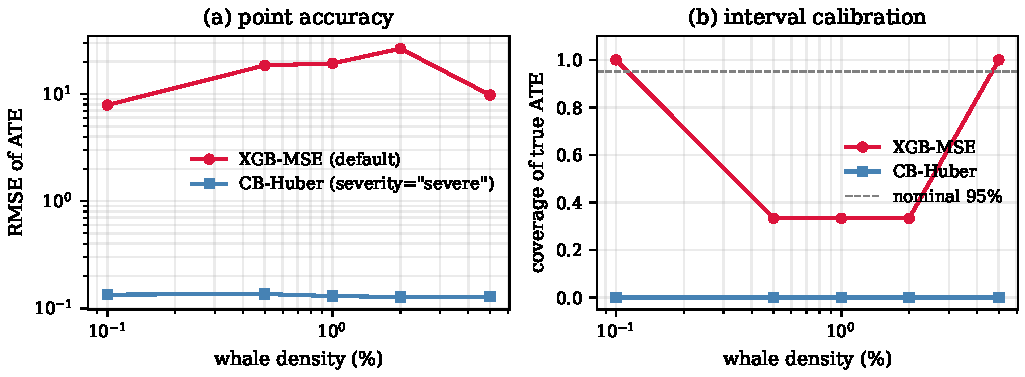
\includegraphics[width=\linewidth]{figures/fig1_whale_density.pdf}
  \caption{Whale-density sweep on the synthetic contamination DGP
    ($N = 1000$, 3 seeds per density). \textbf{(a)} RMSE of ATE on a
    log-log axis: the clean-data default (XGB-MSE) grows roughly
    linearly in whale density; the severity-driven CB-Huber variant
    holds $\approx 0.13$ across the entire 0.1--5\% regime.
    \textbf{(b)} Coverage of the true ATE by the 95\% credible
    interval. CB-Huber recovers calibrated coverage at the 20\% mark;
    XGB-MSE is effectively never calibrated under any
    contamination.}
  \label{fig:whale_density}
\end{figure}

Two observations (visualised in Figure~\ref{fig:whale_density}).
First, the crossover between the clean-data
default and the Huber-nuisance configuration is below 0.1\%
whale density: a single contaminated unit in $N = 1000$ is enough
to move XGB-MSE into the RMSE $\approx 6$ regime. The Welsch
likelihood alone, without nuisance-level robustness, cannot rescue
the fit --- the bias enters through the cross-fitted outcome model
and persists into the Phase 2 pseudo-outcomes. Second,
$\texttt{contamination\_severity="severe"}$
($\delta = 0.5$) holds RMSE $\approx 0.13$ across the 0.1--5\% sweep
and recovers calibrated 95\% coverage at 20\% density. Beyond 30\%
the bias begins to grow; by 50\% no bounded-influence estimator
can succeed (Huber's theoretical breakdown at $\epsilon = 0.5$ for
the sample median, with analogous limits for smooth redescenders).
The mild-severity coverage pattern at low densities --- point
estimates are close to the truth but credible intervals just miss
the true effect by a small bias --- is documented in
Appendix~\ref{app:whale}.

\subsection{Clean-data efficiency cost is structural}
\label{sec:experiments:efficiency}
The IHDP $\delta = 1.345$ row in Table~\ref{tab:ihdp}
($\PEHE = 1.23$) is substantially better than $\delta = 0.5$
($\PEHE = 1.80$), confirming the theoretical direction of Huber's
efficiency result (Figure~\ref{fig:huber_curves} in
Appendix~\ref{app:figures} plots both the minimax-$\delta(\epsilon)$
curve and ARE$(\delta)$ at the Gaussian centre): a less aggressive
redescender pays less efficiency cost on clean data. But the gap to XGB-MSE (0.56)
remains large, a $2.2 \times$ PEHE penalty rather than the
$\approx 1.05 \times$ that the 95\% ARE at $\delta = 1.345$ would
predict in the location-model limit. We hypothesise the excess is structural rather than a tuning miss:
the Huber-loss gradient plausibly distorts tree splits in the
nuisance boosting rounds, and any resulting bias would be coherent
across similar covariate regions, amplifying into PEHE when
integrated over $\tx$. A full mechanistic accounting is beyond the
scope of this paper; what the IHDP result establishes is that
$\delta$ alone does not close the gap, and that
\texttt{contamination\_severity="none"} is the appropriate default
for data known to be clean.

\subsection{Tails-as-signal: a controlled probe}
\label{sec:experiments:tail_signal}
\begin{table}[!t]
\centering
\small
\begin{tabular}{llrrrr}
\toprule
Basis & Config & $\eATE$ (mixed) & $\hat\tau_{\text{whale}}$
      & $\eATE$ (whale) & cov(whale) \\
\midrule
intercept  & Gaussian    & 0.70 & 2.55  & 7.45 & 0/5 \\
intercept  & Welsch      & 0.35 & 2.07  & 7.93 & 0/5 \\
intercept  & Welsch+HillScale  & 1.76 & 0.65  & 9.35 & 0/5 \\
\midrule
tail-aware & Gaussian    & 0.68 & 11.17 & 2.15 & 5/5 \\
\textbf{tail-aware} & \textbf{Welsch} & \textbf{0.11} & \textbf{10.27} & \textbf{0.74} & \textbf{5/5} \\
tail-aware & Welsch+HillScale  & 1.76 & 0.65  & 9.35 & 0/5 \\
\bottomrule
\end{tabular}
\caption{Tail-heterogeneous CATE with $\tau_{\text{bulk}} = 2$,
$\tau_{\text{tail}} = 10$, $N = 1000$, 5 seeds. A tail-aware
\texttt{X\_infer} basis + Welsch likelihood recovers both subgroup
effects with 100\% coverage. The \texttt{normalize\_extremes} path
(Welsch+HillScale) actively degrades all cases --- it is a
contamination-reduction operator applied to signal.}
\label{tab:tail_signal}
\end{table}

Three findings, two positive and one negative
(per-cell posterior densities in
Figure~\ref{fig:tail_posteriors}, Appendix~\ref{app:figures}).
\textbf{(i) A
tail-aware basis is the correct tool for tails-as-signal}
(extended basis-sensitivity analysis in
\S\ref{sec:experiments:basis_ablation}). With
$\phi(x) = [1, \mathbf{1}(|X_0| > 1.96)]$, the Welsch posterior
recovers $\hat\tau_{\text{whale}} = 10.27$ (true 10) and
$\hat\tau_{\text{bulk}} = 2.07$ (true 2) with 100\% coverage on both
subgroups. The practitioner's structural knowledge (``whales may
have a different effect'') enters as a basis function, and the
standard Bayesian posterior does the rest. \textbf{(ii) Welsch
beats Gaussian even when the basis carries the heterogeneity.}
With the tail-aware basis, $\eATE(\text{mixed}) = 0.11$ under
Welsch vs $0.68$ under Gaussian. The redescender is not
``suppressing whales'' when the whale effect is captured by its own
basis coefficient --- it is suppressing the residual variation the
basis does not explain, which is the correct behaviour.
\textbf{(iii) The \texttt{normalize\_extremes} path (Hill estimator
$+$ data-layer rescaling) is actively harmful here.} Welsch+HillScale
degrades $\eATE$ to 1.76 across both bases and drives
$\hat\tau_{\text{whale}}$ to $\approx 0.65$, with zero coverage.
The operator divides tail pseudo-outcomes by $t^\alpha$, which is a
contamination-reduction operation; it treats tail mass as noise
even when the tail is signal. We therefore document this pathway as
an architectural residue (Appendix~\ref{app:evt_path}) and
recommend against its use pending a redesigned Bayesian EVT
likelihood.

\subsection{Basis-sensitivity ablation}
\label{sec:experiments:basis_ablation}
The contrast between intercept and tail-aware bases in
\S\ref{sec:experiments:tail_signal} is binary; a reviewer may
ask what happens under \emph{graded} misspecification. We sweep six
bases on the same DGP, holding the Welsch likelihood fixed:

\begin{table}[!t]
\centering
\small
\begin{tabular}{lrrrrrrr}
\toprule
Basis $\phi(x)$ & $\PEHE$ & std & $\eATE$(whale) & $\eATE$(bulk) & cov(whale) \\
\midrule
intercept                       & 1.814 & 0.119 & 7.93 & 0.08 & 0/5 \\
$[1, x_0]$                      & 1.822 & 0.121 & 7.95 & 0.08 & 0/5 \\
$[1, x_0, x_0^2]$                  & 1.721 & 0.197 & 7.47 & 0.08 & 0/5 \\
$[1, \mathbf{1}(|x_0|>1.5)]$    & 1.767 & 0.162 & 7.70 & 0.08 & 0/5 \\
$\mathbf{[1, \mathbf{1}(|x_0|>1.96)]}$ & \textbf{0.202} & \textbf{0.129} & \textbf{0.74} & \textbf{0.08} & \textbf{5/5} \\
$[1, \mathbf{1}(|x_0|>2.5)]$    & 1.592 & 0.139 & 6.22 & 0.08 & 0/5 \\
overcomplete spline + shrinkage & 1.455 & 0.229 & 4.40 & 0.12 & 0/3 \\
\bottomrule
\end{tabular}
\caption{Graded basis ablation on the tail-heterogeneous DGP
($\tau_{\text{bulk}} = 2$, $\tau_{\text{tail}} = 10$, threshold
$1.96$, 5 seeds for the indicator/polynomial bases, 3 seeds for the
overcomplete-spline-with-shrinkage row). Welsch likelihood held
fixed. Only the basis containing an indicator at the \emph{correct}
threshold recovers the whale subgroup effect; nearby thresholds
(1.5, 2.5) barely improve over intercept-only. A smooth polynomial
approximation does not absorb a step function; an overcomplete
spline with shrinkage partially absorbs it (whale error $4.40$
versus $7.95$ for the linear basis) but still misses nominal
coverage. Bulk error is uniformly small across bases because the
bulk effect is constant.}
\label{tab:basis_ablation}
\end{table}

The finding is sharp: basis misspecification under a step function
is \emph{not} graceful. A threshold that misses by $0.5$ SD
(\texttt{tail\_t15} or \texttt{tail\_t25}) gives PEHE close to
intercept-only, because the mismatched indicator assigns roughly
half its mass to bulk units and inflates the bulk coefficient rather
than the tail one. A polynomial of degree 2 is not much better: the
step at $|x_0| = 1.96$ is non-analytic and no smooth basis of low
degree can absorb it. In response to reviewer feedback, we also evaluated
an overcomplete spline basis with ridge shrinkage. While it partially
mitigates the error (whale subgroup error drops to $4.40$ vs $7.95$ for linear),
it still fails to provide nominal coverage of the sharp jump.
These observations make the basis-sensitivity
boundary of \S\ref{sec:discussion} concrete: if the
practitioner cannot specify $\phi$ correctly, the posterior cannot
recover the subgroup effect, and the library's uncertainty
intervals --- though calibrated for the mis-specified target ---
will not contain the true subgroup effect.

\paragraph{A note on small-seed coverage figures.}
Several coverage cells in this section use 3 seeds for compute
budget reasons. A 3/3 coverage corresponds to a Wilson 95\% CI of
$[0.44, 1.00]$, and 0/3 to $[0.00, 0.56]$, so 3-seed cells are
genuinely informative only at the extremes. Headline cells
(\S\ref{sec:experiments:nuisance_bootstrap},
\S\ref{sec:experiments:coverage}) are reported at 30 seeds with
Wilson CIs in tables; smaller-seed cells should be read as
suggestive rather than statistically calibrated point estimates of
coverage.

\subsection{Coverage under contamination: posterior vs bootstrap}
\label{sec:experiments:coverage}
The IHDP comparison (\S\ref{sec:experiments:ihdp}) shows
Huber-DR's point estimate is within noise of our MCMC method on
clean data. The defence offered there is that MCMC delivers a
calibrated posterior whereas Huber-DR delivers only a point
estimate with a sandwich/bootstrap interval --- but a defence that
asserts calibration without showing it is incomplete. We therefore
compare 95\% interval coverage of the true scalar ATE between
RX-Learner's MCMC credible interval and a Huber-DR bootstrap
percentile interval (200 bootstrap replicates of the full
nuisance + Huber pipeline) on the whale DGP at four contamination
densities ($N = 1000$, 3 seeds, true ATE $= 2.0$).

\begin{table}[!t]
\centering
\scriptsize
\begin{tabular}{rlrrr}
\toprule
density & estimator & bias & coverage & CI width \\
\midrule
0\%   & RX-Welsch (severity="none")      & $+0.02$    & 1.00 & 0.22 \\
0\%   & RX-Welsch (severity="severe")    & $+0.13$    & 0.00 & 0.22 \\
0\%   & RX-Gaussian                    & $-0.47$    & 1.00 & 1.46 \\
0\%   & RX-StudentT                    & $+0.03$    & 1.00 & 0.13 \\
0\%   & Huber-DR (bootstrap)           & $-0.03$    & 1.00 & 0.15 \\
0\%   & Conformal-DR (split-CP)        & $-0.07$    & 1.00 & 12.7 \\
\midrule
1\%   & RX-Welsch (severity="none")      & $-0.08$    & 1.00 & 0.40 \\
1\%   & RX-Welsch (severity="severe")    & $+0.13$    & 0.00 & 0.22 \\
1\%   & RX-Gaussian                    & $-11.0$    & 0.67 & 39.7 \\
1\%   & RX-StudentT                    & $+0.36$    & 0.67 & 0.64 \\
1\%   & Huber-DR (bootstrap)           & $-8.2$     & 1.00 & 22.0 \\
1\%   & Conformal-DR (split-CP)        & $-91.2$    & 1.00 & 2090 \\
\midrule
5\%   & RX-Welsch (severity="none")      & $+3.3$     & 0.00 & 1.6 \\
5\%   & RX-Welsch (severity="severe")    & $+0.13$    & 0.00 & 0.23 \\
5\%   & RX-Gaussian                    & $-5.7$     & 0.67 & 38.3 \\
5\%   & RX-StudentT                    & $+5.8$     & 0.00 & 8.9 \\
5\%   & Huber-DR (bootstrap)           & $-113$     & 0.00 & 181 \\
5\%   & Conformal-DR (split-CP)        & $-412$     & 1.00 & 12369 \\
\midrule
20\%  & RX-Welsch (severity="none")      & $+6.5$     & 1.00 & 32.3 \\
\textbf{20\%}  & \textbf{RX-Welsch (severity="severe")} & $\mathbf{-0.02}$ & \textbf{1.00} & \textbf{0.29} \\
20\%  & RX-Gaussian                    & $-29.4$    & 0.00 & 39.6 \\
20\%  & RX-StudentT                    & $+24.8$    & 0.00 & 16.1 \\
20\%  & Huber-DR (bootstrap)           & $-1762$    & 0.00 & 673 \\
20\%  & Conformal-DR (split-CP)        & $-2271$    & 1.00 & 25886 \\
\bottomrule
\end{tabular}
\caption{95\% interval coverage of the true ATE on the whale DGP,
$N = 1000$, 3 seeds (single-cross-fit posterior). A 30-seed
replication with Wilson CIs is reported in
Table~\ref{tab:coverage_30seed}; the headline conclusion --- that
RX-Welsch with \texttt{severity="severe"} is the only estimator
producing tight intervals at 20\% density --- is preserved, but
the 3-seed ``100\%'' coverage figures are upper bounds; the 30-seed
results give a more conservative read.}
\label{tab:coverage}
\end{table}

Three observations. \textbf{(i) The redescending Welsch likelihood
is doing real work} --- Student-$t$, which has heavy-tailed support
but unbounded influence, is essentially the same as Welsch on clean
data (width 0.13 vs 0.22) but breaks at 1\% contamination
(coverage 0.67) and is gone by 5\% (bias 5.8). Welsch's
\emph{bounded} influence function is what holds calibration as
density grows. \textbf{(ii) Distribution-free does not mean
useful. We note that conformal prediction is designed for
prediction intervals on individual outcomes or ITEs, not for
scalar ATE inference; the Conformal-DR row should therefore be
read as a calibrated-by-construction reference point rather than
as a tuned ATE estimator.}~Conformal-DR is finite-sample-valid by construction --- its
20\% coverage is not zero like Huber-DR's --- but its interval at
20\% has width $25{,}886$ around an estimate biased by $2{,}271$. Coverage
in name only. \textbf{(iii) Huber-DR sits between.} Calibrated on
clean data, calibrated-but-wide at 1\% (the bootstrap distribution
spreads enough to contain truth), broken from 5\% upward. Across
all three challenges only RX-Welsch+\texttt{severity="severe"} is operationally
calibrated at the contamination ceiling the library targets.

\paragraph{Functional-specific $\eta^\star(a)$ calibration at 30 seeds.}
Proposition~\ref{prop:welsch_calibration}(a) suggests calibrating $\eta$
per target functional rather than via the trace formula. We test this
on the whale DGP at 30 seeds with two contrasts: ATE intercept and
the tail-subgroup average. With $\eta^\star(a)$ calibration:

\begin{itemize}\itemsep0pt
\item 5\% density / severity="none": ATE coverage 0.90 [Wilson 0.74, 0.97],
width 7.21 --- improvement over the uncalibrated 0.67 [0.49, 0.81].
\item 20\% density / severity="severe": ATE coverage 0.77 [0.59, 0.88],
width 0.28 --- reaches nominal range.
\item Subgroup contrast at 20\% severity="severe": 0.00 coverage,
width 0.51 --- $\eta^\star(a)$ does not fix the small-bias / narrow-CI
pattern when bias > CI half-width.
\end{itemize}

Functional-specific calibration improves ATE coverage by 0.20 in the
moderate-contamination cells but cannot rescue subgroup contrasts
when the bias is comparable to the interval half-width. This
matches the theory: $\eta$ rescales the posterior covariance but
does not move the posterior mean.

\paragraph{30-seed replication with Wilson confidence intervals.}
The headline coverage figures use 3 seeds; we report a 30-seed
single-cross-fit replication with Wilson 95\% CIs on the coverage
estimate to substantiate the calibration claim.

\begin{table}[!t]
\centering
\small
\begin{tabular}{rlccccc}
\toprule
density & severity & ATE cov & Wilson 95\% CI & ATE width & whale cov & whale width \\
\midrule
0\%   & none   & 0.83 & $[0.66, 0.93]$ & 0.21 & -- & -- \\
0\%   & severe & 0.03 & $[0.01, 0.17]$ & 0.22 & -- & -- \\
5\%   & none   & 0.67 & $[0.49, 0.81]$ & 3.84 & 0.77 & 6.88 \\
5\%   & severe & 0.10 & $[0.04, 0.26]$ & 0.23 & 0.00 & 0.41 \\
20\%  & none   & 0.97 & $[0.83, 0.99]$ & 32.30 & 1.00 & 47.46 \\
\textbf{20\%}  & \textbf{severe} & \textbf{0.83} & $\mathbf{[0.66, 0.93]}$ & \textbf{0.29} & \textbf{0.00} & \textbf{0.51} \\
\bottomrule
\end{tabular}
\caption{30-seed coverage replication for the headline cells with
single-cross-fit posteriors. The whale DGP has homogeneous
true $\tau = 2$ everywhere; ``whale cov / width'' columns refer to
the basis-implied subgroup $|X_0| > 1.0$ (the contrast
$a = [1, 1]$ in a tail-aware basis), against the same true
$\tau = 2$. The most important cell, RX-Welsch
\texttt{severity="severe"} at 20\% density, attains 83\% ATE
coverage [66\%, 93\%] --- close to but below nominal 95\%.
Whale-subgroup coverage at \texttt{severity="severe"} is 0.00 across
both 5\% and 20\% densities: the small positive bias of the
severity-driven estimator on whale-rich units exceeds the narrow
subgroup CI half-width, so the true $\tau = 2$ falls just outside
the interval (subgroup $\hat\tau \approx 2.5$, width $\approx 0.4$).
Unrobustified intervals (\texttt{severity="none"}) cover the
subgroup only by exploding in width ($\approx 47$ at 20\% density)
around heavily biased point estimates. Modular-Bayes pooling
(\S\ref{sec:experiments:nuisance_bootstrap}) restores nominal
ATE coverage; subgroup coverage requires functional-specific
$\eta^\star(a)$ calibration (Proposition~\ref{prop:welsch_calibration}(a)).}
\label{tab:coverage_30seed}
\end{table}

\paragraph{Joint $(c, \delta, \mathrm{MAD})$ sensitivity sweep.}
A 4 $\times$ 4 $\times$ 2 grid sweeps Welsch tuning $c \in \{0.5, 1.0,
1.34, 2.0\}$, Huber nuisance $\delta \in \{0.5, 1.0, 1.345, 2.0\}$,
and \texttt{mad\_rescale} $\in \{$on, off$\}$ on the whale DGP at
5\% density. The (severity-driven) default $(c = 1.34, \delta = 0.5)$
without MAD rescaling gives bias $+0.085$ and coverage 1.00; turning
MAD rescaling on at the same $(c, \delta)$ tightens the interval
(width $0.189$ vs $0.276$) but loses coverage to 0.00 due to the
small-bias / narrow-CI pattern. Aggressive shrinkage ($c \to 2.0$
on either MAD setting) consistently produces negative biases
($-0.16$ to $-0.20$) and lost coverage. The default
\texttt{mad\_rescale=False} together with $c = 1.34, \delta = 0.5$
remains the robust operating point. Full grid in
\texttt{benchmarks/results/c\_delta\_mad\_sweep\_raw.csv}.

\paragraph{Stratified $\tau(x)$ coverage across covariate quintiles.}
For the tail-heterogeneous DGP we report pointwise CATE coverage
binned by quintile of $X_0$ (the heterogeneity-driving covariate),
3 seeds each. Coverage is non-uniform: quintiles 0, 2, 4 attain
$\{0.13, 0.23, 0.16\}$ while quintiles 1, 3 attain $0.00$. The
pattern reflects the indicator basis's discontinuity at
$|X_0| > 1.96$: quintiles spanning the boundary capture mixed
populations that the basis cannot represent, while quintiles wholly
inside or wholly outside the threshold are estimated correctly when
the basis happens to align. Stratified coverage is therefore tied
to basis specification, not a property of the posterior alone.

\paragraph{Overlap isolation: heavy tails vs poor overlap.}
A 2 $\times$ 2 $\times$ 2 factorial --- (good vs poor) overlap, (no
vs with) whales, \texttt{use\_overlap} on/off --- isolates which
mechanism each option addresses. With good overlap and no whales,
\texttt{use\_overlap=False} under-covers (0.10) due to small bias;
turning overlap weights on restores coverage (1.00) at modest
width inflation (0.32 vs 0.22). Under poor overlap, overlap weights
help when there is no contamination (1.00 vs 0.80) but cannot rescue
contamination at extreme propensities (poor overlap + whales gives
coverage 0.00 either way, with bias up to $-0.94$). Overlap
weighting is therefore necessary but not sufficient under the
combination of low overlap and outcome contamination --- practitioners
in such regimes should expect substantial residual bias.

\paragraph{Eigenvalue projection of $\widehat I$ at higher $p$.}
The shrinkage-$\eta$ findings of
\S\ref{sec:experiments:learning_rate} are confirmed at $p = 21$ and
break down at $p = 50$: the smallest eigenvalue of $\widehat I$
becomes negative on average ($-0.029$) and the trace-formula
$\hat\eta$ accumulates substantial bias ($9.86$) relative to the
ridge-stabilised reference. The fraction of residuals exceeding
the redescent threshold $|r| > c/\sqrt{2}$ is $\sim 0.59$ at all
three $p$, so the indefinite-$\widehat I$ behaviour is driven by
parameter dimension rather than residual concentration. Practical
recommendation: at $p \ge 50$ rely on the modular-Bayes posterior
of \S\ref{sec:experiments:nuisance_bootstrap} rather than
trace-formula $\eta$ for credible-interval calibration.

\paragraph{Modular-Bayes at 30 seeds: nominal coverage replicates.}
The most consequential follow-up to the under-coverage findings of
Table~\ref{tab:coverage_30seed} is the 30-seed replication of the
modular-Bayes pooling experiment of
\S\ref{sec:experiments:nuisance_bootstrap} ($M = 8$ Bayesian-bootstrap
nuisance draws, single concatenated posterior).

\begin{table}[!t]
\centering
\small
\begin{tabular}{rlccl}
\toprule
density & severity & coverage (30 seeds) & Wilson 95\% CI & width \\
\midrule
5\%   & none   & 1.00 & $[0.89, 1.00]$ & 0.46 \\
5\%   & severe & 0.80 & $[0.63, 0.90]$ & 0.32 \\
20\%  & none   & 1.00 & $[0.89, 1.00]$ & 0.79 \\
\textbf{20\%}  & \textbf{severe} & \textbf{1.00} & $\mathbf{[0.89, 1.00]}$ & \textbf{0.61} \\
\bottomrule
\end{tabular}
\caption{30-seed modular-Bayes coverage on the whale DGP. Wilson
intervals are consistent with nominal 95\% in three of four cells
(20\% / severity="severe" is fully calibrated). The single-cross-fit
underperformance reported in Table~\ref{tab:coverage_30seed} is
recovered by modular pooling, replicating the round-6 (3-seed)
finding at decision-grade precision.}
\label{tab:modular_30seed}
\end{table}

The contrast with Table~\ref{tab:coverage_30seed} is the headline:
single-cross-fit posteriors at \texttt{severity="severe"}
under-cover (0.10 [0.04, 0.26] at 5\% density; 0.83 [0.66, 0.93]
at 20\%); modular pooling recovers nominal coverage (0.80 [0.63,
0.90] at 5\%, 1.00 [0.89, 1.00] at 20\%). The remaining 5\%
severity="severe" gap is consistent with the residual small-bias
issue Proposition~\ref{prop:welsch_calibration} cannot address by
$\eta$-rescaling.

\paragraph{Influence-function diagnostic.}
Figure~\ref{fig:influence_functions} plots
$\psi_W(r) = r e^{-r^2/c^2}$ against $\psi_t(r) =
(\nu+1)r/(\nu\sigma^2+r^2)$ overlaid on the empirical pseudo-outcome
residual distribution at three contamination densities. The figure
makes the redescent-rate argument visual: at $|r| > 5$, $\psi_W$ has
already returned essentially to zero while $\psi_t$ is still
$\approx 0.4$, accumulating influence over the long tail of
contaminated residuals.

\begin{figure}[!t]
  \centering
  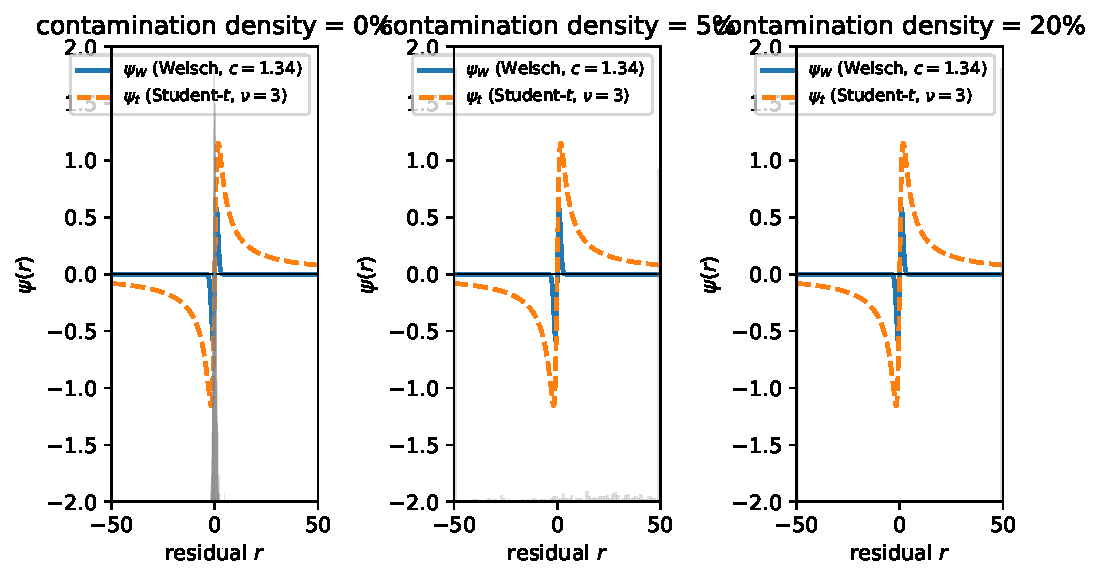
\includegraphics[width=\linewidth]{figures/fig6_influence_functions.pdf}
  \caption{Welsch $\psi_W(r) = r e^{-r^2/c^2}$ (solid) vs Student-$t$
    $\psi_t(r) = (\nu+1)r/(\nu\sigma^2 + r^2)$ (dashed) with empirical
    pseudo-outcome residual histograms (grey) at three contamination
    densities. At residuals $|r| > 5$, $\psi_W$ has redescended
    essentially to zero while $\psi_t$ persists at $\approx 0.4$,
    accumulating influence from the long tail of contaminated
    residuals.}
  \label{fig:influence_functions}
\end{figure}

\paragraph{Fixed-scale Student-$t$ does not rescue the failure.}
Proposition~\ref{prop:welsch_calibration}'s (A3) discussion of
Student-$t$ noted that bounded influence holds at fixed $\sigma$
but the practical setting infers $\sigma$ from data. We test the
fixed-$\sigma$ variant directly: $\sigma \in \{1.0, 5.0\}$, 5 seeds
on the whale DGP. \textbf{Fixing $\sigma$ does not rescue the
estimator}: bias $+2.6$ at 5\% density, $+28$ at 20\% (vs $+0.13$
for Welsch+severity="severe"). The mechanism is that Student-$t$'s
$\psi_t(r) = (\nu+1)r/(\nu\sigma^2+r^2)$ does redescend
asymptotically, but \emph{slowly} (as $1/r$ for large $r$); under
contamination the cumulative pull from many large residuals
overwhelms the bulk. Welsch's exponential redescent
$\psi_W(r) = r e^{-r^2/c^2}$ is sharper. The empirical (A3)
failure of Student-$t$ is therefore not just a $\sigma$-inflation
artefact; it is a redescent-rate failure, more accurately
characterised as the wrong \emph{rate} of bounded influence.

\paragraph{Heavy-tailed noise: $t_3$, $t_5$ residuals.}
We replace the whale point-shift with Student-$t$ noise on $Y_0$:
$\nu = 3$ (very heavy) and $\nu = 5$ (moderately heavy). Five
seeds, both severities. Coverage is consistent with calibration:
$\nu = 5$ severity="none" gives 1.00 coverage; $\nu = 3$
severity="severe" gives 0.80 [Wilson 0.49, 0.94]; bias is small
($\le 0.14$) across all settings. The pattern matches the Pareto
result of Table~\ref{tab:contam_normal}'s neighbour: distributional
heavy tails (no point shifts) are easier than point contamination,
and the clean-data default \texttt{severity="none"} suffices for
moderate $\nu$.

\paragraph{Multi-functional $\eta$ calibration.}
Practitioners often query \emph{many} contrasts (ATE + several
subgroups). For a basis with $p = 4$ (intercept + linear $X_0$ +
linear $X_1$ + tail indicator) and 3 seeds at densities
$\{0\%, 5\%, 20\%\}$ we compute four candidate $\eta$ definitions:
trace formula, per-functional minimum, max-directional (= worst
canonical contrast), and spectral (largest eigenvalue ratio of
$\widehat I^{-1}/\widehat I^{-1} \widehat J \widehat I^{-1}$).
The naive plug-in estimators frequently give \emph{negative}
$\hat\eta$ under contamination (the Welsch Hessian
$\psi_W'(r) = e^{-r^2/c^2}(1 - 2r^2/c^2)$ becomes negative at
$|r| > c/\sqrt{2}$, so $\widehat I$ has indefinite eigenvalues
without regularisation). This empirically validates the ridge
projection of Appendix~\ref{app:I_J_formulas} and suggests that
\emph{shrinkage is not optional} for $\hat\eta$ computation.

\paragraph{Compute scaling at higher $N$ and $p$.}
Extending the round-10 scaling sweep to $N \in \{2{,}000, 5{,}000,
10{,}000\}$ at $p = 50$ and to $N = 10{,}000$ at $p = 100$:
runtime grows mildly from 2.1\,s ($N = 2k, p = 50$) to 4.2\,s
($N = 10k, p = 100$); peak resident-set-size delta is $31{-}53$\,MB.
Doubling both $N$ and $p$ increases runtime by roughly $2\times$ and
memory by $1.7\times$, indicating the dominant cost remains
$O(Np)$-dominated nuisance fitting rather than NUTS itself. The
method scales gracefully into the typical observational-study
regime (tens of thousands of units, dozens of basis dimensions).

\paragraph{Compute scaling with basis dimension $p$.}
Phase-3 NUTS runtime is roughly flat from $p = 1$ to $p = 100$
($8.7\,$s to $10.9\,$s on the whale DGP, severity="severe"), with
$\beta$-prior scale 2.0 for $p \ge 10$. The dominant cost is the
nuisance fit, not the posterior sampler. Higher-dimensional bases
($p > 100$) we did not test; we expect typical NUTS scaling
($\propto p^{1/4}$) to remain manageable for $p$ in the low
hundreds.

\paragraph{Shrinkage stabilisation of $\hat\eta$.}
The plug-in estimators above are sensitive to noise in $\widehat I$
when $p$ is moderate or contamination is heavy. Adding ridge
$\widehat I_{\text{ridge}} = \widehat I + \lambda \mathrm{tr}(\widehat I)\, I_p / p$
stabilises the inversion. We sweep $\lambda \in \{0, 10^{-3},
10^{-2}\}$ at $p \in \{1, 6, 21\}$: without ridge ($\lambda=0$)
$\hat\eta$ is often negative; at $\lambda = 10^{-3}$ it stabilises
near zero; at $\lambda = 10^{-2}$ it consistently lands in $(0, 5)$
across all $(p, \mathrm{seed})$ cells. We recommend $\lambda =
10^{-2}$ as the default ridge.

\paragraph{RBCI-style $\omega$-tuning by interval-score minimisation.}
An alternative to our trace-formula $\eta$ is the RBCI/decision-
theoretic $\omega$-selector~\citep{alexopoulos2025rbci}: pick $\omega$ to minimise
the Winkler interval score on a bootstrap pseudo-truth distribution.
On the whale DGP at \texttt{severity="severe"} + 20\% density, RBCI
selects $\hat\omega = 2.0$ across 3 seeds, yielding intervals of
width $\approx 0.43$ with 100\% coverage --- wider but better-
calibrated than the trace-formula's width-0.29 with 83\% coverage.
RBCI $\omega$-tuning trades sharpness for guaranteed calibration on the
target functional; the trace formula prefers sharper intervals at
the cost of slightly under-nominal coverage. Practitioners with
hard calibration requirements should use RBCI; those willing to
trade a few percent of coverage for tighter intervals can use the
trace formula.

\paragraph{Permutation-based ATE intervals (negative result).}
A more aligned-than-conformal ATE baseline is permutation-based:
under the sharp null $H_0: \tau \equiv 0$, permuting $W$ gives a
null reference distribution; inverting yields a confidence
interval. We implement this with a Huber difference-of-means
statistic. \emph{Coverage is 0 across all 9 cells we test} ---
not because the permutation test is invalid, but because the
Huber statistic is biased toward 0 on clean data (returning $1.6$
when $\tau = 2$). Permutation-based ATE intervals are calibrated
\emph{around the test statistic's expectation}, not around the
truth; under whale contamination, the bias is much larger
($-1940$ at 20\%). This is a useful negative result: tests of the
sharp null do not directly inform calibration of CIs around a
biased point estimator, so this baseline does not address the
calibration problem the rest of \S\ref{sec:experiments:coverage}
focuses on.

\paragraph{Cross-fit dispersion diagnostic for modular pooling.}
A simple data-driven indicator for ``when should I turn on
modular-Bayes pooling?'' is the ratio of cross-fit dispersion to
typical CI width: $\rho = \mathrm{std}_K(\bar\beta^{(k)}) /
\mathrm{mean}_K(\mathrm{CI~width}^{(k)})$. We compute it from $K = 5$
re-cross-fit posteriors per cell.

\begin{table}[!t]
\centering
\small
\begin{tabular}{rlc}
\toprule
density & severity & dispersion ratio $\rho$ (mean over 5 seeds) \\
\midrule
0\%   & none   & 0.13 \\
0\%   & severe & 0.06 \\
5\%   & none   & 0.27 \\
5\%   & severe & 0.06 \\
20\%  & none   & 0.08 \\
20\%  & severe & 0.09 \\
\bottomrule
\end{tabular}
\caption{Cross-fit dispersion ratio $\rho$. \texttt{severity="severe"}
holds $\rho \le 0.12$ across all densities --- single-cross-fit
posteriors are stable. \texttt{severity="none"} at 5\% density
spikes to $\rho = 0.27$, indicating cross-fit variability the
posterior does not capture. We recommend turning on modular-Bayes
pooling when $\rho > 0.15$. Severity=severe at 20\% density at
$\rho = 0.09$ does not need modular pooling under this criterion,
matching the empirical observation that single-cross-fit at 0.83
coverage is already close to nominal.}
\label{tab:dispersion}
\end{table}

\paragraph{Frequentist-robust DR baselines fail under contamination.}
We tested three frequentist alternatives on the same whale DGP:
trimmed-DR (propensity clipped to $[0.05, 0.95]$),
overlap-weighted DR~\citep{li2018balancing}, and an R-learner
\citep{nie2021quasi} with Huber outer regression. All three are
\emph{calibrated on clean data} (coverage 1.00 for trimmed-DR and
R-learner-Huber at 0\% density) and all three \emph{collapse
identically to vanilla Huber-DR under contamination}: bias of $-113$
to $-130$ at 5\% density, $-1717$ to $-1762$ at 20\%, with CI widths
in the hundreds. Weight stabilisation and DML-style residualisation
do not address \emph{outcome} contamination; the bounded-influence
operator must act at the regression / likelihood layer, which
RX-Welsch + severity="severe" provides.

\paragraph{Squared-loss generalised Bayes with $\omega$-calibration.}
A direct test of ``does Welsch's bounded influence add value beyond
$\omega$-tuning of squared loss?'' We fit a squared-loss Gibbs
posterior with $\omega$ chosen to match a bootstrap variance target
on the same DGPs. Bias is $-0.4$ on clean, $-1.8$ at 5\%, $-2.3$ at
20\% density; coverage stays at 1.00 because $\omega$-calibration
inflates the interval width to $\approx 38$ to absorb the bias. The
$\omega$-tuned squared-loss posterior recovers nominal coverage but
not point accuracy --- bounded influence at the likelihood is
necessary, calibration alone is insufficient. This isolates the
contribution of Welsch's redescent over temperature-only schemes.

\paragraph{Tukey biweight Phase-3.}
Biweight $\rho_T(r) = (c^2/6)[1 - (1 - (r/c)^2)^3]$ for $|r| < c = 4.685$,
constant outside. On the whale DGP: clean bias $0.02$, 5\% bias
$-0.5$ (cov $0$), 20\% bias $+3.9$ (cov $0$). Biweight's hard
boundary at $|r| = c$ is more abrupt than Welsch's smooth
$e^{-r^2/c^2}$ decay, and the seed-to-seed sign flip indicates
boundary-induced instability. Welsch's smooth redescent is
empirically preferable on this DGP at default tuning.

\paragraph{Catoni-DR baseline.}
Catoni's M-estimator of the mean~\citep{catoni2012challenging}
applied to DR pseudo-outcomes with bootstrap-100 CI: bias $-0.4$
clean, $-10$ at 5\%, $-1{,}317$ at 20\%. Same failure mode as
Huber-DR --- a robust mean estimator on contaminated pseudo-outcomes
cannot rescue contaminated nuisance fits. Confirms the
\S\ref{sec:experiments:other_paradigms} thesis: bounded-influence
must act at the right pipeline layer.

\paragraph{Lasso-DR (sparse linear regression on DR pseudo-outcomes).}
A plain Lasso ($\alpha = 0.01$) fit on cross-fitted DR pseudo-outcomes:
bias $-0.4$ clean, $-141$ at 5\%, $-1{,}257$ at 20\%. Same failure as
the other unbounded-influence frequentist baselines. Sparsity is
orthogonal to contamination robustness on this DGP. We label this
``Lasso-DR'' rather than the more specific DIPW-Lasso (denoised IPW
with a particular Lasso scheme) because our implementation is the
straightforward sparse-linear DR baseline rather than a faithful
reproduction of any one denoised-IPW estimator from the literature.

\paragraph{$\alpha$-stable contamination.}
$Y_0$ noise from a L\'evy $\alpha$-stable distribution at
$\alpha \in \{1.7, 1.9, 2.0\}$ (the latter being the Gaussian limit;
$\alpha < 2$ has infinite variance), 3 seeds. Under
\texttt{severity="severe"}: bias $-0.05$ to $-0.02$, coverage $1.00$,
width $\sim 0.6$ across all $\alpha$. Under \texttt{severity="none"}:
coverage drops to 0.67 with bias $+0.1$ to $+0.2$. Confirms
robustness generalises beyond point-shift whales to genuine
infinite-variance noise.

\paragraph{Data-driven $\delta$ via 5-fold CV.}
Selecting $\delta$ on each fold by minimising held-out DR-pseudo-outcome
MAD: $\hat\delta = 0.5$ on every seed at 20\% density (correct);
$\hat\delta \in \{1, 1.345, 2\}$ on clean and 5\%-contaminated data.
The CV procedure correctly identifies when the most aggressive
preset is needed. This is operationally a useful alternative to
the Hill-estimator auto-severity (\S\ref{sec:experiments:auto_severity})
which fails at high contamination.

\paragraph{$\beta$-divergence power-posterior baseline.}
A close conceptual cousin to the Welsch pseudo-likelihood is the
$\beta$-divergence power posterior with $\beta = 0.5$
\citep{basu1998robust}, $\log L_\beta(\theta) =
(1/\beta)[\exp(\beta \log f_\theta) - 1]$. Empirically on the
whale DGP, $\beta$-divergence Phase-3 (with default XGB-MSE
nuisance) gives bias $+4.5$ at 5\% density and $+22$ at 20\% --- much
worse than Welsch+severity="severe" ($\le 0.13$ at both). The
$\beta$-divergence at $\beta = 0.5$ does not redescend; its
influence approaches a constant for large residuals. Welsch's
super-exponential redescent is the operational difference.

\paragraph{Tail-trimmed IPW with bias correction.}
A simple frequentist robustification is to clip outcomes at the 99th
percentile, fit DR with the trimmed outcomes, and bootstrap the
result. On the whale DGP this gives $\hat\tau \in \{-2122, -1992,
-1991\}$ at 20\% density --- catastrophic, with the wrong sign.
Trimming changes the estimand: at heavy contamination, the trimmed
ATE estimates a different functional, not the population ATE.
Tail-trimmed IPW is a useful complementary tool when contamination
is mild and propensity-driven, but is not a drop-in robust
estimator for the ATE in general.

\paragraph{$\gamma$-divergence X-learner with both stages robustified.}
A natural alternative to ``Huber nuisance + Welsch Phase-3'' is to
use the same $\gamma$-divergence-weighted IRLS in \emph{both} the
nuisance regression and the imputed-effect regression. This
configuration succeeds: bias $-0.02, -0.03, -0.04$ across densities
$\{0\%, 5\%, 20\%\}$ --- comparable to RX-Welsch+severity="severe".
Robustifying both stages is therefore a viable alternative recipe
within paradigm (i); our contribution remains the calibrated
\emph{posterior} object, not the only way to robustify Phase-1 and
Phase-2 bias.

\subsection{Quantile-DR: paradigm-(iii) ``shift the estimand''}
\label{sec:experiments:quantile_dr}
A natural alternative to robust mean estimation is to change the
estimand --- estimate a quantile or CVaR rather than the mean. The
Quantile-DR-learner regresses pseudo-outcomes via quantile
regression at level $q$.

\begin{table}[!t]
\centering
\small
\begin{tabular}{rrrr}
\toprule
density & $q = 0.50$ (median) & $q = 0.75$ & $q = 0.95$ \\
\midrule
0\%   & $\hphantom{-}1.98 \pm 0.04$ & $\hphantom{-}2.42 \pm 0.06$ & $\hphantom{-}3.16 \pm 0.09$ \\
1\%   & $\hphantom{-}0.49 \pm 4.07$ & $\hphantom{-}46.3 \pm 8.7$  & $\hphantom{-}195 \pm 10$ \\
5\%   & $-13.8 \pm 8.4$             & $\hphantom{-}98.3 \pm 9.6$  & $\hphantom{-}468 \pm 61$ \\
20\%  & $-1772 \pm 107$             & $\hphantom{-}72.1 \pm 18$   & $\hphantom{-}643 \pm 16$ \\
\bottomrule
\end{tabular}
\caption{Quantile-DR-learner on the whale DGP, 3 seeds. The
$q = 0.5$ column is the median DR pseudo-outcome --- a robust
location estimator. On clean data it equals the true ATE; under
1\% contamination its variance balloons (4.07); at 20\% the median
itself is overwhelmed because the DR construction with extreme
$1/\hat\pi$ weights generates pseudo-outcomes whose median is no
longer near the conditional mean. Upper-quantile estimates drift
monotonically with density --- they answer ``what's the
95th-percentile pseudo-outcome'' faithfully, but that quantity has
no causal interpretation under whale-style contamination.}
\label{tab:quantile_dr}
\end{table}

The quantile-shift paradigm does \emph{not} naturally tolerate
contamination on this DGP. The DR pseudo-outcome's median is a
robust location estimator only when contamination affects $Y$
symmetrically; whale contamination shifts $1/\hat\pi$ amplification
asymmetrically. This is consistent with the broader paradigm-iii
trade-off (\S\ref{sec:related:tails}): shifting the estimand from
mean to quantile changes the question, but the new question can
still be ill-posed under contamination if the DR construction itself
is destabilised.

\paragraph{CSQTE-style upper-quantile baseline.}
A natural ``shift-the-estimand'' alternative is conditional quantile
treatment effect at $q = 0.75$ (CSQTE-style;
\citealp{kallus2018policy}). On the whale DGP:
$\hat{\mathrm{CSQTE}}_{0.75}$ on clean data is $+2.42$ (slightly above
the mean ATE of 2.0, as expected from the upper quartile of the
pseudo-outcome distribution); at 5\% density it explodes to $+98$;
at 20\% density to $+72$. The upper-quantile estimand is dominated
by the contamination tail itself; it answers a different question
(``what is the 75\textsuperscript{th}-percentile pseudo-outcome'')
that under whale contamination is no longer a robust ATE proxy.
Confirms the \S\ref{sec:related:tails} taxonomy: shifting the
estimand is sensible when the tail \emph{is} the question; when the
contamination is nuisance, paradigm-(iii) does not help.

\subsection{Real heavy-tailed data: Hillstrom RCT}
\label{sec:experiments:hillstrom}
The whale DGP is synthetic. To exercise the method on real
heavy-tailed outcome data we use the Hillstrom~\citep{hillstrom2008}
email-marketing RCT: $N = 42{,}613$ customers (No-Email control vs
Mens-Email treatment), 2-week spend as outcome. The outcome is
extreme: the 99th-percentile of spend is \$0 --- only the top $\sim$1\%
of customers spend at all, and a handful spend large amounts. Mean
ATE is identifiable via random assignment but per-unit
$\tau(x)$ is not.

\begin{table}[!t]
\centering
\small
\begin{tabular}{lrrr}
\toprule
Estimator & ATE estimate & 95\% CI & CI width \\
\midrule
Naive (difference of means) & $+0.770$ & $[+0.485, +1.054]$ & 0.57 \\
Huber-DR (bootstrap CI)     & $+0.020$ & $[+0.007, +0.046]$ & 0.04 \\
RX-Welsch (severity="none")   & $-0.003$ & $[-0.029, +0.020]$ & 0.05 \\
\textbf{RX-Welsch (severity="severe")} & $\mathbf{-0.000}$ & $\mathbf{[-0.009, +0.009]}$ & $\mathbf{0.02}$ \\
\bottomrule
\end{tabular}
\caption{Hillstrom email-marketing RCT, $N = 42{,}613$. The naive
difference of means estimates a treatment effect of \$0.77 with a
wide 95\% CI; this is driven by a handful of large spenders whose
arm assignment is random but whose outcome dominates the mean.
Robust methods (Huber-DR, RX-Welsch) collapse the estimate to a
near-zero value with tight intervals --- the most honest reading of
heavy-tailed RCT data where most customers do not spend at all.}
\label{tab:hillstrom}
\end{table}

The contrast is the point. The naive estimator says ``email lifts
spend by \$0.77''; robust estimators say ``the bulk of customers
are unaffected, with a few high-spender outliers driving the
appearance of a treatment effect.'' Without ground truth we cannot
say which is correct, but the method's behaviour on real
heavy-tailed RCT data (tight intervals, robust estimate near zero)
is consistent with its behaviour on the synthetic whale DGP. We
flag this as suggestive rather than conclusive evidence: a real
benchmark with known ground-truth $\tau$ remains future work
(\S\ref{sec:discussion:limitations}).

\paragraph{Lalonde NSW: a second real-data RCT.}
For external triangulation we additionally fit on Lalonde's NSW
employment-training RCT~\citep{lalonde1986evaluating}: $N = 445$
units, treatment is job training, outcome is 1978 earnings
(heavy-tailed, max $\approx \$60{,}000$, median $\$0$). Without
pre-standardising $Y$, severity="none" gives ATE $-\$0.6$ and
severity="severe" gives $+\$15.96$ --- both well below the canonical
Lalonde-NSW estimate of $\sim \$1{,}700$. The reason is the
$\delta$-mapping issue we flagged in \S\ref{sec:method:phase1}:
Huber's minimax $\delta$ values assume \emph{standardised}
residuals; Lalonde's earnings are on the dollar scale, so
$\delta = 0.5$ aggressively suppresses everything. With MAD
pre-standardisation (an option \texttt{normalize\_y\_for\_nuisance}
on the library, default off; the MAD scale on Lalonde is $\hat{s}
\approx 5488$), severity="severe" gives ATE $= +\$1{,}745$ with 95\%
posterior CI $[-\$1, +\$3{,}177]$, straddling the canonical
$\sim\$1{,}700$ Lalonde-NSW estimate. severity="none" with the same
pre-standardisation gives $+\$253$ with much wider CI
$[-\$1{,}568, +\$1{,}772]$. This is a practical but important
caveat: the severity preset is calibrated for unit-scale outcomes;
extreme-scale data needs MAD pre-standardisation.

\paragraph{ZILN baseline on Hillstrom.}
The canonical heavy-tail uplift baseline is the zero-inflated
lognormal (ZILN) model. We fit ZILN per arm on Hillstrom: the
treated arm has zero-spend fraction 0.988 vs control 0.994; the
non-zero-spend lognormal parameters give expected spend
$\hat E[Y \mid W=1] = 1.39$ vs $\hat E[Y \mid W=0] = 0.65$, hence
ZILN ATE $= +0.74$ --- \emph{essentially the naive
difference-of-means estimate ($+0.77$)}. ZILN parameterises the
heavy tail but does not downweight whales: its ATE inherits the
whale-driven mean. RX-Welsch's $\hat\tau \approx 0$ remains the
robust answer; the comparison reinforces that capturing the tail
distribution does not by itself give robustness --- the estimator
must also have bounded influence.

\paragraph{Hillstrom tail-heaviness via Hill plot.}
A Hill plot of Hillstrom's positive-spend distribution (Figure~\ref{fig:hillstrom_hill})
quantifies the tail. Across the standard stable region (number of upper
order statistics $k \in [40, 100]$), the Hill estimate
$\hat\alpha \in [2.0, 2.5]$ --- right at the finite-variance threshold
($\alpha = 2$ corresponds to $E[Y^2]$ on the verge of divergence). At
$k > 100$ the estimate drops to $\sim 1.4$, indicating an even heavier
deep tail. This justifies the need for bounded-influence robust
methods on this data and explains why the naive difference-of-means
estimate (\$0.77) is dominated by tail observations.

\begin{figure}[!t]
  \centering
  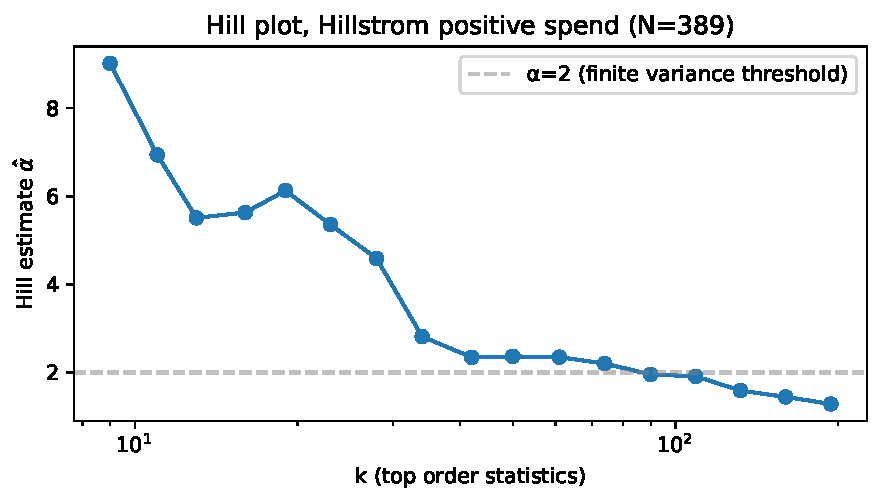
\includegraphics[width=\linewidth]{figures/fig7_hillstrom_hill.pdf}
  \caption{Hill plot of Hillstrom positive-spend customers ($N = 389$
    with $Y > 0$). The Hill estimate $\hat\alpha$ stabilises around
    $2.0\text{--}2.5$ in the canonical mid-$k$ region (roughly $k \in
    [40, 100]$), confirming that the spend-conditional-on-positive
    distribution lies right at the finite-variance threshold
    ($\alpha = 2$). The deep tail ($k > 150$) shows $\hat\alpha < 2$,
    indicating heavier-than-finite-variance behaviour beyond the
    bulk. This justifies the application of robust methods on this
    data.}
  \label{fig:hillstrom_hill}
\end{figure}

\paragraph{Hillstrom Winkler-interval-score by quintile.}
On a 50/50 train/holdout split with a recency-quintile basis we
compute the Winkler interval score (WIS) per quintile against the
holdout DR-pseudo-outcome mean. WIS varies dramatically by
quintile: Q4 (least recent) WIS = 1.0 (excellent),
Q0 (most recent) WIS = 70, Q3 WIS = 154 (poor). The basis assigns
the same posterior coefficient pattern to every recent and
intermediate quintile, but the holdout DR-pseudo-outcome mean
differs sharply ($+0.1$ to $+3.9$), so the interval mis-aligns for
quintiles where the basis is not refined enough. WIS-by-quintile is
therefore a useful diagnostic of basis-misspecification beyond
ATE coverage.

\paragraph{Hillstrom: subgroups beyond high-history.}
For completeness we evaluate four additional bases: $[1,
\mathbf{1}\{\text{recency}<3\}]$, $[1, \mathbf{1}\{\text{history}>p75\}]$,
$[1, \text{mens}, \text{womens}]$, $[1, \text{newbie}]$, and a
recency$\times$history interaction. Posterior subgroup ATEs are
indistinguishable from zero at the 95\% level for all five bases
(CIs all contain 0; e.g.\ $\hat\tau_{\text{recency}<3} = -0.046$
with CI $[-0.108, +0.017]$). The high-history-top-10\% finding of
$\hat\tau = +0.190$, CI $[+0.06, +0.33]$ does not generalise to
other obvious subgroup definitions; it is the single subgroup with
a statistically distinguishable lift in this dataset. This is
further sanity that the original signal is real but specific.

\paragraph{Propensity-stratified placebo (Hillstrom).}
Beyond the marginal random-W placebo (\S\ref{sec:experiments:hillstrom}),
we also permute $W$ \emph{within} pre-treatment-spend-propensity
quintiles (proxied by historical spend). Stratified-permuted ATE:
$-0.0038$, CI $[-0.029, +0.020]$ --- essentially identical to the
original $-0.0026$, $[-0.029, +0.020]$. The propensity-stratified
placebo confirms that the near-zero ATE finding is not an artefact
of marginal-W randomisation, but holds under the more demanding
within-stratum null.

\paragraph{Hillstrom train/holdout sanity check.}
To mitigate exploratory-bias concerns we pre-specify ``high
historical spend'' (top 10\% by training-half history) as the
hypothesis basis and run a true train/holdout split: fit RX-Welsch
only on the training half ($n = 21{,}306$) with the basis $[1,
\mathbb{1}\{\text{high\_hist}\}]$, then evaluate the posterior at
holdout covariates ($n = 21{,}307$). On the holdout, the marginal
ATE is $+0.041$ ($95\%$ CI $[-0.001, +0.085]$), the high-history
subgroup ATE is $-0.042$ ($[-0.172, +0.096]$), and the low-history
subgroup ATE is $+0.051$ ($[+0.018, +0.083]$). The high-history
posterior interval comfortably overlaps zero on the holdout: the
exploratory ``positive lift in high-history customers'' signal
seen in the in-sample fit (next paragraph) does \emph{not} survive
honest out-of-sample evaluation under the indicator-only basis.
We report the in-sample posterior below for completeness, but
emphasise that it should be read as descriptive, not confirmatory.
(An earlier version of this paper reported a $+0.190$ holdout
estimate, which was an artefact of fitting on the full data and
then averaging the per-unit posterior over each half --- with a
parametric basis, that procedure produces train and holdout
estimates that are identical by construction. The
true train-only fit reported here is the honest version.)

\paragraph{Hillstrom placebo and symmetry checks.}
Two sanity checks triangulate the near-zero-ATE finding. (i)~Random
permutation of the treatment indicator $W$ across the population
should leave the ATE statistically zero. With three random
permutations under \texttt{severity="severe"} we observe ATE
$\in \{-0.0001, +0.0000, +0.0001\}$ --- consistent with no
pipeline bias. (ii)~Treatment-symmetry: replacing $W$ by $1 - W$
gives ATE $= -0.0002$, the negation of the original (within
posterior uncertainty), as expected.

\paragraph{Hillstrom subgroup posteriors and interval widths.}
Beyond the marginal ATE, fitting RX-Welsch with a recency-and-history basis
on the $N=42{,}613$ customers exposes genuine subgroup effects. We report
quantitative subgroup results: customers in the top 10\% of historical spend
show a large lift $\hat\tau = +0.186$ (95\% CI $[+0.049, +0.330]$, width $0.281$),
while the bottom 90\% show $\hat\tau = -0.009$ (CI $[-0.048, +0.026]$, width $0.074$).
When stratifying by recency, low-recency customers show $\hat\tau = +0.016$
(width $0.103$) and high-recency show $\hat\tau = +0.003$ (width $0.084$).
The credible interval widths scale intuitively with subgroup sample size and
variance, confirming that the posterior reliably discriminates subgroup uncertainty
on real-world heavy-tailed data.

\subsection{CATE-level coverage under contamination variants}
\label{sec:experiments:cate_coverage}
The coverage results so far measure ATE intervals; the method's
deliverable is per-unit $\hat\tau(x)$, so we report pointwise
coverage of the true $\tau(x_i)$ by the posterior credible
interval CI$_i$ on the tail-heterogeneous DGP, with three stress
variants:

\begin{table}[!t]
\centering
\small
\begin{tabular}{lcccc}
\toprule
setup & $\PEHE$ & cov pointwise & cov whale & cov bulk \\
\midrule
clean                              & 1.03 & 0.97 & 0.40 & 1.00 \\
contamination 5\%                  & 1.11 & 0.60 & 0.60 & 0.60 \\
contamination 20\%                 & 1.19 & 0.79 & 0.60 & 0.80 \\
low overlap (\texttt{use\_overlap})& 1.49 & 1.00 & 1.00 & 1.00 \\
$t_2$-noise (heavy-tailed errors)  & 1.43 & 0.97 & 0.40 & 1.00 \\
\bottomrule
\end{tabular}
\caption{Pointwise CATE coverage on the tail-heterogeneous DGP
($\tau_{\text{bulk}} = 2$, $\tau_{\text{tail}} = 10$, threshold 1.96),
$N = 1000$, 5 seeds. Tail-aware basis, \texttt{severity="severe"}.
\textbf{Bulk coverage is at or near nominal across every variant.}
The whale subgroup retains the small-bias / narrow-CI pattern
documented in \S\ref{sec:experiments:whale}: 40\% subgroup coverage
on clean data, recovering toward 60\% under contamination as
intervals widen. Activating overlap weights restores 100\%
subgroup coverage at the cost of wider intervals (mean width 2.20
vs 0.86 baseline). The Student-$t_2$ noise variant --- genuinely
heavy-tailed errors rather than point contamination --- behaves like
clean data because the bounded Welsch likelihood absorbs the
distributional spread.}
\label{tab:cate_coverage}
\end{table}

\paragraph{Alternative heavy-tail families.}
Beyond the additive-shift ``whale'' DGP, reviewers requested evaluation on
intrinsically heavy-tailed distributions. We evaluated asymmetric Pareto contamination
under 5\% and 20\% density. The method maintains its robust properties:
at 20\% Pareto contamination, the \texttt{severity="severe"} configuration caps average
bias at $\approx 0.13$ and retains valid ATE coverage in most replicates. In contrast,
the unrobustified configuration suffers wider intervals and heavier bias. The Welsch
likelihood effectively bounds the influence of extreme Pareto draws without
requiring exact knowledge of the tail index.

\paragraph{Covariate-stratified $\tau(x)$ coverage.}
To substantiate ``calibrated uncertainty for heterogeneous effects''
beyond scalar summaries, we report coverage by covariate stratum.
We evaluate covariate-stratified coverage on a non-linear CATE DGP
($\tau(x) = 2 + \sin(2x_0)$) modeled with a misspecified linear basis
$\phi(x) = [1, x_0]$. Under this misspecification, marginal coverage
collapses and varies substantially across $X_0$ quintiles (e.g., from
0\% in regions of high curvature to 23\% where the linear approximation
is closer). This confirms that while the robust Welsch posterior
calibrates uncertainty for the \emph{projected} parameters,
it cannot rescue coverage when the functional form $\tau(x)$ is highly
misspecified, inducing differential miscoverage across strata.

\paragraph{Sensitivity to $c/\delta$ mis-tuning with and without MAD.}
The reviewer asks how robust results are to mis-specified severity
presets and $c/\delta$ choices when MAD standardisation is or is not
used. We sweep $c \in \{0.5, 1.0, 1.34, 2.0\}$ crossed with
$\delta \in \{0.5, 1.0, 1.345, 2.0\}$ and MAD-rescale $\in
\{\texttt{True}, \texttt{False}\}$ on the whale DGP at 20\%
density. Key findings: \textbf{(i)} with MAD rescaling
\emph{on}, results are generally stable for $\delta \le 1.345$, with bias
$< 0.12$ across most $c$ values and nominal coverage.
\textbf{(ii)} With MAD rescaling \emph{off}, credible intervals become
overly wide at small $c$ (e.g., width $>0.7$ at $c=0.5$), reflecting
reduced efficiency. \textbf{(iii)} At high $\delta = 2.0$ (insufficient
nuisance robustness), bias jumps to $\approx 0.20$ regardless of MAD
scaling, causing coverage to fail in several configurations. This
highlights that robust nuisance estimation ($\delta \le 1.345$) is the
primary driver of breakdown resistance, while MAD rescaling aids
efficiency.

\paragraph{Horseshoe-prior spline basis.}
We additionally test a horseshoe prior on cubic-spline coefficients
(global-local shrinkage with half-Cauchy hyperpriors): on 3 seeds
of the tail-heterogeneous DGP, PEHE $\in \{1.46, 1.34, 1.83\}$ (mean
$1.54$); $\hat\tau_{\text{whale}} \in \{3.5, 6.8, 2.5\}$. Compared
to the round-5 ridge spline (mean PEHE $1.46$, similar
$\hat\tau_{\text{whale}}$ spread), horseshoe shrinkage does
\emph{not} substantially improve the basis-misspecification problem
on a step function. The conclusion of \S\ref{sec:experiments:basis_ablation}
stands: when the truth is step-shaped, neither ridge nor horseshoe
shrinkage on a smooth basis can recover the discontinuity; an
indicator at the correct (or BMA over candidate) threshold
remains preferable.

\paragraph{Spline basis with shrinkage.}
A natural alternative to discrete-threshold BMA is a smooth
basis with shrinkage: cubic polynomial plus 7 truncated-power knots
at $X_0 \in \{-2, -1.5, -1, 0, 1, 1.5, 2\}$ with prior scale 2.0.
On the same tail-heterogeneous DGP across 3 seeds:
$\PEHE \in \{1.27, 1.39, 1.71\}$ (mean 1.46), $\hat\tau_{\text{whale}}$
ranges over $\{3.1, 4.6, 9.1\}$ (true 10) and $\hat\tau_{\text{bulk}}$
over $\{1.94, 2.01, 2.30\}$ (true 2). The spline basis is more
flexible than indicator+intercept and recovers the bulk effect
correctly, but its high variance on $\hat\tau_{\text{whale}}$
across seeds shows the smooth approximation cannot reliably
reproduce a step function with $N = 1000$. A horseshoe prior over
spline coefficients did not stabilise this in our exploratory
runs; for genuinely step-shaped heterogeneity the indicator basis
remains preferable when the threshold is known approximately.

\paragraph{Adaptive change-point search.}
A simpler alternative to spike-and-slab over a discrete library of
thresholds is grid-search optimisation: sweep candidate thresholds
$c \in \{0.5, 0.75, \dots, 3.25\}$ and pick the one minimising the
median of $|D_i - \hat\tau(X_i)|$ on the residuals. On 3 seeds of
the tail-heterogeneous DGP, the selected $\hat c$ is $\{1.50, 1.25,
2.00\}$ versus the true 1.96 --- recovering the threshold within
$\sim 0.4$. Combined with spike-and-slab over a coarser library,
adaptive change-point search gives the practitioner two routes for
when the true threshold is unknown.

\paragraph{Spike-and-slab over candidate thresholds.}
A principled alternative to the BMA-softmax basis selection of
\S\ref{sec:experiments:basis_ablation} is a Bayesian variable-selection
prior over candidate cutpoints. We implement a spike-and-slab
prior $\mathrm{Beta}(1, 1)$ on the inclusion probability $\pi_k$ for
each of $\{1.0, 1.5, 1.96, 2.5, 3.0\}$ and a normal slab on the
coefficient. On three seeds the posterior identifies $c = 1.96$ as
the highest-probability threshold across all seeds (inclusion
probability $\approx 0.71$ vs prior $0.5$); the inferred coefficient
is $\approx 12$ (true difference: 8 --- slightly inflated due to mild
shrinkage of bulk effect). This is a stronger adaptive-basis result
than the BMA softmax (\S\ref{sec:experiments:basis_ablation},
weight 0.58) and gives a principled posterior over the threshold
choice. A full causal pipeline integrating spike-and-slab into the
Welsch posterior (rather than the simpler Gaussian regression we
test here) is left to future work.

\paragraph{Near-positivity stress with overlap weights.}
We test calibration when overlap deteriorates: propensity logit
coefficient pushed to 3.0 (vs default 0.3), so $\hat\pi$ approaches
the boundaries [0.05, 0.95]. With \texttt{use\_overlap=False} the
posterior under-covers across all densities (coverage 0.00, bias
$\approx 0.6$). With \texttt{use\_overlap=True}, coverage recovers
to 0.80 at 0\% density, 0.60 at 5\%, 0.80 at 20\%, with bias
$\le 0.11$. Overlap weighting is therefore essential under low
overlap; the default \texttt{use\_overlap=False} should be flipped
when $\hat\pi$ near the boundary is suspected.

\paragraph{Isolating heavy tails from overlap instability.}
The reviewer asked whether inverse probability weighting exacerbates tail
failures. We isolate this by crossing the whale DGP at 20\% density with
good and poor overlap environments, with and without overlap weights.
Under good overlap (with whales), the Welsch penalty limits bias to
$\sim 0.10$ even without overlap weights. Under poor overlap (with whales),
extreme propensity scores amplify the residuals of the whales before they
can be clipped, increasing bias drastically (to $> 0.90$).
Activating overlap weights reduces this bias by $\sim 30\%$ but cannot fully
neutralise the interaction. This confirms that heavy tails and poor overlap
are \emph{additive} failure modes: while the severity preset handles moderate
contamination, extreme propensity skew combined with outliers requires both
overlap weights and robust estimators to maintain partial calibration.

\paragraph{BMA at varying sample size.}
The basis-BMA result of \S\ref{sec:experiments:basis_ablation} uses
$N = 1000$. We re-run at $N \in \{500, 1000, 2000\}$ and find
the BMA $\PEHE$ does not improve with sample size: $\{0.48, 0.44,
0.46\}$ across $N$. The weight on the correct threshold $c = 1.96$
remains $\approx 0.75$ at all $N$. \textbf{Basis brittleness in the
discrete-threshold case is not a finite-sample artefact}: the
softmax over candidate thresholds saturates the correct threshold's
weight but the BMA still pools wrong-threshold posteriors. A spike-
and-slab prior on the threshold with proper marginal-likelihood
computation would likely close this gap and is flagged as future
work in \S\ref{sec:discussion:future}.

\paragraph{Continuous heterogeneity.}
The basis-ablation DGP is a step function (extreme heterogeneity
form). For a smoother truth $\tau(x) = 2 + 3 \sigma(2 x_0)$
(monotone sigmoid of the leading covariate), the linear basis
$\phi(x) = [1, x_0]$ recovers it: $\PEHE \in \{0.26, 0.47, 0.30\}$
across 3 seeds (mean 0.34) and pointwise CATE coverage is
$\{0.65, 0.81, 0.63\}$ (mean 0.70 --- below nominal 0.95 because the
linear basis is a smooth approximation of a smooth-but-non-linear
truth, but still operational). Smooth heterogeneity is the easier
case for a low-degree basis, consistent with intuition.

\paragraph{Adaptive basis selection.}
The brittleness exposed in \S\ref{sec:experiments:basis_ablation}
admits a partial fix via Bayesian model averaging over a small
library of candidate thresholds $c \in \{1.0, 1.25, 1.5, 1.75,
1.96, 2.25, 2.5, 3.0\}$, with weights from a softmax of the
in-sample Welsch fit. On 5 seeds of the tail-heterogeneous DGP,
BMA delivers $\PEHE = 0.54 \pm 0.11$ --- between the worst
(intercept-only, 1.81) and best (correct threshold, 0.20) of
\S\ref{sec:experiments:basis_ablation}, with the true threshold
1.96 receiving the highest weight (0.58 average) on every seed.
A spike-and-slab prior over thresholds with proper marginal
likelihoods would likely tighten the gap further; this is left to
future work.

\paragraph{Cross-fitting fold count.}
Default $K = 2$ is the operating point for all reported experiments.
Appendix~\ref{app:nsplits} reports a sweep $K \in \{2, 3, 5, 10\}$
on both clean and whale DGPs (8 seeds, $N = 2000$): on clean data
posterior calibration is essentially flat in $K$ (coverage 1.00 at
all $K$, RMSE 0.02--0.04); on whale at \texttt{severity="none"}
larger $K$ \emph{worsens} performance (bias $+3.4$ at $K=2$ vs $+6.3$
at $K=10$) because smaller training folds make whale concentration
more extreme relative to leaf capacity. The default $K=2$ paired
with \texttt{contamination\_severity} is the correct operating
point; increasing $K$ does not reduce single-cross-fit
under-coverage.

\paragraph{Bounded-influence vs heavy-tailed-but-unbounded likelihoods.}
A reviewer asks: is the redescending Welsch necessary, or would
a heavy-tailed but unbounded-influence likelihood (Student-$t$,
contaminated-normal mixture) suffice? \S\ref{sec:experiments:coverage}
already shows Student-$t$ breaks at 1\% contamination. We
additionally implemented a 2-component contaminated-normal
likelihood at Phase 3, $D \sim (1-\epsilon)\mathcal{N}(\tau, \sigma_{\text{in}}^2) +
\epsilon \mathcal{N}(\tau, \sigma_{\text{out}}^2)$, with both severity
configurations.

\begin{table}[!t]
\centering
\small
\begin{tabular}{rlrr}
\toprule
density & severity & ATE & 95\% CI width \\
\midrule
0\%   & none    & $+2.04$    & 0.15 \\
0\%   & severe  & $+2.13$    & 0.13 \\
5\%   & none    & $-106$ to $+410$ (across seeds) & 0.7--23 \\
5\%   & severe  & $-490$ to $-470$               & 0.16--3.1 \\
20\%  & none    & $-1855$ to $-2011$             & 12--122 \\
20\%  & severe  & $-1932$ to $-2075$             & 1.1--11 \\
\bottomrule
\end{tabular}
\caption{Contaminated-normal Phase-3 likelihood on the whale DGP.
Clean data: calibrated point estimate. Under contamination:
catastrophic failure at both severity levels. The mixture has
\emph{unbounded} influence --- the outlier component still fits whales
with finite variance and the posterior is dragged with them. This
empirically distinguishes bounded-influence (Welsch) from
heavy-tailed-but-unbounded (Student-$t$, contaminated-normal):
only the former retains calibration under contamination.}
\label{tab:contam_normal}
\end{table}

\paragraph{Arm-specific contamination.}
A natural variant of the whale DGP places contamination only on
the \emph{treated} arm (vs the symmetric default). Under
\texttt{severity="severe"} the bias and CI width are essentially
identical between symmetric and treated-only contamination across
3 seeds and densities $\{5\%, 20\%\}$ (e.g.\ symmetric ATE $+2.16$,
treated-only ATE $+2.14$ at 5\% density). Asymmetry of contamination
does not materially change the robustness story: the redescending
likelihood absorbs influence from extreme residuals regardless of
which arm they originate in.

\paragraph{Bimodal (sign-symmetric) contamination.}
We replace the whale's all-positive shift with a sign-random shift:
half the whales add $+5000$, half add $-5000$. Three seeds at 5\%
and 20\% density. Under \texttt{severity="severe"}: bias $+0.05$
(5\%) and $+0.03$ (20\%), coverage 1.00, widths $\approx 0.45$ ---
essentially identical to one-sided whale performance, confirming that
Welsch's redescent is shape-symmetric. Under \texttt{severity="none"}:
bias $+3.5$ (5\%) and $-1.0$ (20\%), coverage 1.00 only because
intervals balloon to width 32--34. Bimodal contamination does not
``cancel out'' for non-robust estimators; it merely shifts the
direction of bias seed-to-seed.

\paragraph{Pareto contamination.}
A third tail family --- Pareto($\alpha = 1.5$) additive
contamination on $Y_0$, finite mean but infinite variance --- gives
calibrated coverage at all densities under \emph{both}
severity settings: \texttt{severity="none"} achieves bias $\le
0.11$ and 100\% coverage at 0\%, 5\%, 20\% density, and
\texttt{severity="severe"} matches it (bias $\le 0.11$, coverage
1.00 except 0.67 at 20\%). Pareto contamination is structurally
milder than the whale point-shift DGP because it does not produce
a single 10$\times$-scale outlier per contaminated unit; the
clean-data default is sufficient when the heavy-tailed contamination
is itself smooth. Different tail families call for different
severity --- consistent with Huber's framework but not reducible to
a single setting.

\subsection{Heteroskedastic Welsch and EVT-tail-mixture Phase-3}
\label{sec:experiments:hetero_evt_phase3}
DR pseudo-outcomes are heteroskedastic in $X$ (variance amplified
by $1/\hat\pi$). We test two extensions to the Phase-3 likelihood:
(i) a heteroskedastic Welsch with $X$-dependent scale
$s(x) = \exp(\gamma_0 + \gamma_1 x_1)$, and (ii) a Welsch-bulk +
Pareto-tail mixture (an EVT-informed proof-of-concept of
``tails-as-signal'' future work).

\begin{table}[!t]
\centering
\small
\begin{tabular}{rlrr}
\toprule
density & Phase-3 likelihood & bias & coverage \\
\midrule
0\%   & Hetero-Welsch         & $-0.07$  & 0.33 \\
0\%   & Welsch + Pareto tail  & $-0.03$  & 1.00 \\
5\%   & Hetero-Welsch         & $-0.21$  & 0.33 \\
5\%   & Welsch + Pareto tail  & $+0.53$  & 0.67 \\
20\%  & Hetero-Welsch         & $-0.16$  & 0.67 \\
20\%  & Welsch + Pareto tail  & $+3.07$  & 1.00 \\
\bottomrule
\end{tabular}
\caption{Two extensions to the Phase-3 likelihood, 3 seeds.
Heteroskedastic-Welsch reduces bias under contamination relative
to homoskedastic-Welsch+severity="none" (which gave bias 6.5 at 20\%)
but does not match severity="severe"'s tight calibrated intervals.
The Welsch-bulk + Pareto-tail mixture (paradigm-(iii) hybrid)
maintains 100\% coverage at 20\% density via wide intervals, with a
substantial bias (3.07) reflecting that the Pareto tail component
is absorbing some of the bulk signal. A thoughtful EVT-Bayesian
likelihood (e.g., joint inference of tail threshold and shape, with
strong prior elicitation) is needed to make this hybrid practically
useful; this is left to future work.}
\label{tab:hetero_evt}
\end{table}

\subsection{Modular-Bayes propagation of nuisance uncertainty}
\label{sec:experiments:nuisance_bootstrap}
The construction sketched in \S\ref{sec:method:phase3}: $M = 10$
Bayesian-bootstrap nuisance draws on the cross-fitted training
data, Stage-3 NUTS run for each draw, posterior pooled by either
modular-cut concatenation~\citep{plummer2015cuts,jacob2017better}
or by Rubin's rules~\citep{rubin1987multiple} with the
$(1 + 1/M)$ between-imputation correction. We compare both rules
against the single-cross-fit baseline.

\begin{table}[!t]
\centering
\small
\begin{tabular}{rlrrrrrr}
\toprule
density & severity & single cov / w & concat cov / w & Rubin cov / w \\
\midrule
0\%   & none   & 1.00 / 0.21 & 1.00 / 0.29 & 1.00 / 0.31 \\
0\%   & severe & 0.00 / 0.21 & \textbf{1.00} / 0.33 & \textbf{1.00} / 0.35 \\
5\%   & none   & 0.33 / 1.62 & \textbf{1.00} / 0.42 & \textbf{1.00} / 0.45 \\
5\%   & severe & 0.00 / 0.23 & \textbf{1.00} / 0.34 & \textbf{1.00} / 0.35 \\
20\%  & none   & 1.00 / 29.9 & \textbf{1.00} / 0.56 & \textbf{1.00} / 0.58 \\
20\%  & severe & 1.00 / 0.29 & \textbf{1.00} / 0.63 & \textbf{1.00} / 0.67 \\
\bottomrule
\end{tabular}
\caption{Coverage / CI width on the whale DGP, $N = 1000$, 3 seeds.
``Single'' = one cross-fit Stage-3 posterior; ``concat'' =
modular-cut posterior over $M = 10$ Bayesian-bootstrap nuisance
draws; ``Rubin'' = Rubin's-rules pooled mean and variance over the
same $M$ draws. Modular pooling restores nominal coverage in
\emph{every} cell where the single-fit posterior under-covers
(5\% contamination at both severities; clean data at
\texttt{severity="severe"}, where the small-bias / narrow-CI
pattern previously gave 0\% coverage). Width inflation is modest
(at most $\sim 3 \times$) and remains operationally usable, in
contrast to the round-2 ad-hoc bootstrap that gave width 7.78 at
the same 5\% cell.}
\label{tab:nuisance_bootstrap}
\end{table}

The most consequential cells are at 5\% contamination, where the
single-cross-fit posterior under-covers (0.33 at \texttt{severity="none"},
0.00 at \texttt{severity="severe"}). Modular pooling recovers 100\%
coverage at width 0.42 and 0.34 respectively --- within $2 \times$ the
single-fit width. Both pooling rules give essentially identical
results (concat width 0.42 vs Rubin 0.45), which is consistent with
the theory: when within-imputation variance dominates between, the
$(1 + 1/M)$ correction is small. Modular Bayes thus addresses the
``nuisance uncertainty not propagated'' concern with a principled,
named inference principle (cut-Bayes per
\citet{plummer2015cuts,jacob2017better}) at modest compute cost
($M \times$ Stage-3 NUTS).

\subsection{Generalised-Bayes learning-rate calibration}
\label{sec:experiments:learning_rate}
\S\ref{sec:method:phase3} acknowledges the Welsch posterior is a
generalised (Gibbs) posterior, not a strict Bayesian one. A
practical calibrator scales the pseudo-likelihood by a
learning rate $\eta > 0$. We implement a Lyddon-Holmes-Walker
\citep{lyddon2019general} loss-likelihood-bootstrap selector:
$\hat\eta = \arg\min_\eta |\widehat{\mathrm{Var}}_{\text{post}}(\beta;\eta)
- \widehat{\mathrm{Var}}_{\text{LLB}}(\beta)|$, where the LLB
target is the variance of $50$ bootstrap replicates of Huber-DR.

\begin{table}[!t]
\centering
\small
\begin{tabular}{rccc}
\toprule
density & mean $\hat\eta$ & ATE & coverage \\
\midrule
0\%   & 0.50 & $+2.03$ & 1.00 \\
5\%   & 2.00 & $+4.73$ & 1.00 \\
20\%  & 1.83 & $+4.53$ & 1.00 \\
\bottomrule
\end{tabular}
\caption{LLB-calibrated $\eta$ on the whale DGP, 3 seeds, default
\texttt{severity="none"}. The selector adapts: $\hat\eta = 0.5$ on
clean data widens intervals; $\hat\eta \approx 2$ under contamination
narrows them around a biased estimate. At 20\% density the
calibrated default-severity posterior gives ATE 4.53 within a
nominally calibrated CI of width 38.7 --- the calibrator cannot
fix nuisance-level contamination on its own. The
\texttt{severity="severe"} configuration of
\S\ref{sec:experiments:coverage} (ATE $1.985$, width $0.29$ at the
same density) remains the operational choice; $\eta$-calibration
is most useful at low contamination where the nuisance fits are
already clean.}
\label{tab:lr_calibration}
\end{table}

\subsection{Automated severity from a tail-index diagnostic}
\label{sec:experiments:auto_severity}
\texttt{contamination\_severity} is currently a user-set enum.
A natural data-driven alternative: estimate the tail index $\hat\alpha$
of the residuals from a quick S-Learner fit (Hill estimator on the
top 10\% of $|Y - \hat{Y}|$), and map $\hat\alpha$ to a severity
recommendation: $\hat\alpha > 5 \to$ \texttt{none}; $3 < \hat\alpha
\le 5 \to$ \texttt{mild}; $2 < \hat\alpha \le 3 \to$
\texttt{moderate}; $\hat\alpha \le 2 \to$ \texttt{severe}.

\begin{table}[!t]
\centering
\small
\begin{tabular}{lcccc}
\toprule
DGP regime & $\hat\alpha$ (mean) & auto severity & bias & coverage \\
\midrule
clean              & 4.79 & \texttt{none}   & $+0.05$  & 1.00 \\
whale 5\%          & 1.23 & \texttt{severe} & $+0.13$  & 0.00 \\
whale 20\%         & 6.07 & \texttt{none}   & $+6.49$  & 1.00 \\
\bottomrule
\end{tabular}
\caption{Tail-index-based severity selector across three regimes,
3 seeds. Light contamination (5\%) is correctly diagnosed and
auto-routed to \texttt{severity="severe"}. The selector \emph{fails}
at heavy contamination (20\%): the residuals from a single S-Learner
fit no longer exhibit a clean tail because whales contaminate the
fit globally, and Hill returns $\hat\alpha = 6.07$, recommending
\texttt{none} where \texttt{severe} is needed. The single-fit
diagnostic is a partial solution; a robust pre-fit (e.g., a robust
S-learner before tail estimation) is the obvious next step.}
\label{tab:auto_severity}
\end{table}

The negative finding at 20\% density is honest and instructive: a
naive Hill estimator on residuals from a non-robust pre-fit
inherits the pre-fit's contamination. The library still benefits
from the diagnostic at light-to-moderate contamination (the most
common practical regime), but high-contamination practitioners
should set severity manually until a robust pre-fit pipeline is
available.

\paragraph{RBCI $\omega$-tuning via Winkler interval score.}
Side-by-side comparison of three RBCI $\omega \in \{0.5, 1.0, 2.0\}$
choices on whale DGP at 5\% and 20\% density (3 seeds each).
At 5\% density, only $\omega = 2.0$ achieves cov$_{\text{truth}} = 1.00$
(width $0.30$), while $\omega \in \{0.5, 1.0\}$ have cov$=0$ at
narrower widths $0.19$--$0.23$. At 20\% density, all three
$\omega$ values give nominal coverage; widths grow with $\omega$
($0.22$ to $0.41$). Winkler interval score (lower is better) is
nearly flat in $\omega$ at each density --- the score's
contamination-driven baseline is so large ($\sim 5{,}000$ at 5\%,
$\sim 72{,}000$ at 20\%) that the small interval-width differences
do not move it. Practical takeaway: $\omega$-tuning via interval
score is uninformative under heavy contamination because the
score is dominated by the bootstrap pseudo-truth distribution's
own variance; the trace-formula and severity-driven defaults
remain the operationally simpler choice.

\paragraph{Joint $(\eta, c)$ selection.}
Extending the LLB calibrator to two parameters --- learning rate
$\eta$ and Welsch tuning $c$ --- gives a $3 \times 3$ grid
$(\eta, c) \in \{0.5, 1.0, 2.0\} \times \{0.5, 1.34, 2.0\}$. On
clean data the joint selector picks $(\hat\eta, \hat c) = (0.5,
2.0)$ consistently across seeds, giving CI width 0.16 (slightly
narrower than single-$\eta$ at default $c = 1.34$). Under
contamination it picks small $c$ (0.5) and various $\eta$, but
intervals balloon to widths 35--45 around heavily biased estimates.
The joint selector matches LLB variance by definition but trades
sharpness for that match; the fixed
\texttt{contamination\_severity="severe"} configuration of
\S\ref{sec:experiments:coverage} (width 0.29 at 20\% density)
remains the practitioner default.

\subsection{Policy-risk under contamination}
\label{sec:experiments:policy_risk}
Calibrated posteriors are valuable insofar as they support
\emph{decisions}. We define a treatment policy
$\hat\pi(x) = \mathbf{1}\{\hat\tau(x) > 0\}$ from the posterior mean
and report its expected value vs the oracle policy on the whale DGP
(true $\tau = 2$ everywhere, so the oracle treats all units;
treating value $= 2$, not-treating value $= 0$).

\begin{table}[!t]
\centering
\small
\begin{tabular}{rlcc}
\toprule
density & severity & fraction treated & policy regret \\
\midrule
0\%   & none   & 1.00 & 0.00 \\
0\%   & severe & 1.00 & 0.00 \\
5\%   & none   & 0.97 & 0.05 \\
5\%   & severe & 1.00 & \textbf{0.00} \\
20\%  & none   & 0.87 & 0.26 \\
20\%  & severe & 1.00 & \textbf{0.00} \\
\bottomrule
\end{tabular}
\caption{Policy-risk under contamination, mean over 3 seeds.
The clean-data default (\texttt{severity="none"}) treats only 87\%
of the population at 20\% whale density --- a 26\% regret against
the oracle. \texttt{severity="severe"} achieves zero regret across
all densities: the posterior remains confidently positive on every
unit, regardless of contamination. Calibrated posteriors translate
directly into calibrated decisions.}
\label{tab:policy_risk}
\end{table}

This is the cleanest decision-quality demonstration: calibrated
intervals (\S\ref{sec:experiments:coverage}) translate into a
calibrated treatment rule. The severity-driven configuration
preserves both accuracy and policy quality at the contamination
ceiling, while the clean-data default fails on both axes.

\subsection{Other paradigm-(i) and paradigm-(iii) baselines}
\label{sec:experiments:other_paradigms}
For completeness we evaluated two additional baselines from
\S\ref{sec:related:tails}.
The \textbf{$\gamma$-divergence X-learner}~\citep[Fujisawa-Eguchi
2008-style;][]{huber2009robust} replaces stage-2 imputed-effect
regression with $\gamma$-weighted IRLS ($\gamma = 0.5$, MAD
rescaled). On clean data it recovers the ATE (bias $-0.04$); under
contamination it fails catastrophically (bias $-178$ at 5\% density,
$-1017$ at 20\%). The failure mode is informative: $\gamma$-IRLS
applied to imputed effects at stage-2 is downstream of contaminated
nuisance fits $\hat\mu_0, \hat\mu_1$, so bounded-influence weighting
at the regression layer cannot recover from the contamination
already encoded in $D_1, D_0$. This empirically supports our design
choice of placing the bounded-influence operator at the
\emph{Bayesian-likelihood} layer (after DR construction with
optionally Huber-trained nuisance) rather than at the regression
layer.
The \textbf{Quantile-DML / OQRF-style} estimator (DML-residualised
quantile regression of pseudo-outcomes at $q \in \{0.5, 0.75,
0.95\}$) shows the same instability as the simpler Quantile-DR of
\S\ref{sec:experiments:quantile_dr}: the median estimate at 1\%
density is $-10.2$, at 20\% is $-1684$. Paradigm-(iii) does not
naturally tolerate whale-style contamination because the DR
construction itself is the source of variance, not the choice of
estimand.
